\section{Introduction}
\label{sec:intro}

% Climate and weather models are expensive, and we really want ensembles
Weather and climate prediction requires the integration of a computational
forecast model, derived from the fundamental equations of motion and initialized
with an estimate of the present-day system state (e.g., temperature, wind speeds,
etc.).
However, knowledge of these initial conditions is imperfect, and the governing
equations contain necessary, inexact approximations of reality.
Thus, reliable climate projections and weather forecasts require an
ensemble of numerical model integrations, where each ensemble member is
initialized with a sample from a prior distribution
representing the uncertainty in the system state.
This process comes at an immense computational cost.
On one hand, it is desirable to increase the credibility of the underlying
numerical model as much as possible,
for instance by increasing model grid resolution
\citep <e.g.,>[]{hewitt_impact_2016}
or by explicitly
simulating as many coupled components (e.g., atmosphere, land, ocean, ice) as
possible \citep <e.g.,>[]{penny_coupled_2017}.
On the other hand, producing an ensemble with reliable statistical significance
requires integrating the underlying numerical model many times; usually
$\mathcal{O}(10-100)$ in practice, but ideally $>1,000$
\citep{evensen_data_2022}.
Therefore, the resulting computational costs require practitioners to trade between the
fidelity of the numerical model and the size of the ensemble.

% Surrogate modeling an encouraging path, and with increased computing power,
% ML, NNs ...
An ongoing area of research that aims to enable statistical forecasting subject
to the dynamics of an expensive numerical model is \textit{surrogate modeling}.
The general approach relies on using a model that represents or ``emulates'' the
dynamics of the original numerical model ``accurately enough'' for the given
application, while being computationally inexpensive to evaluate.
Historically, surrogate models have been developed with techniques like
Linear Inverse Models
\citep <e.g.,
principal oscillation or interaction patterns;>[]{hasselmann_pips_1988,penland_random_1989, moore_linear_2022},
kriging \citep{cressie_statistics_1993},
more general projection based reduced order modeling \citep{bui-thanh_model_2008},
or
polynomial chaos techniques \citep{najm_uncertainty_2009},
to name only a few.
More recently, advances in computing power and the explosion of freely available data
%and more widespread usage of General Purpose Graphics Processing Units (GPGPUs)
has encouraged the exploration of more expensive Machine Learning (ML) methods like
neural networks (NNs) for the emulation task \citep{schultz_can_2021}.
A number of data-driven, NN architectures have been developed to
generate surrogate models for weather forecasting and climate projection
applications, including
feed forward NNs
\citep{dueben_challenges_2018},
Convolutional NNs
\citep <CNNs;>[]{scher_toward_2018,scher_weather_2019,rasp_data-driven_2021,weyn_can_2019,weyn_improving_2020,weyn_sub-seasonal_2021},
Recurrent NNs
\citep <RNNs;>[]{arcomano_machine_2020,chen_predicting_2021,nadiga_reservoir_2021},
Graph NNs \citep{keisler_forecasting_2022},
and Fourier Neural Operators \citep{pathak_fourcastnet_2022}.

%
\begin{table}[]
\caption{
    Recent work using neural networks to emulate processes relevant to weather
    forecasting and climate projection.
}
\label{table:all_the_emulators}

{\footnotesize
\begin{tabular}{c|c|c|c|c|l}
System     & Data Source             & \begin{tabular}[c]{@{}c@{}}Process or\\ Variable\end{tabular} & \begin{tabular}[c]{@{}c@{}}Horizontal\\ Resolution\end{tabular} & Timestep & Citation                                            \\
\hline
Atmosphere & ``Idealized GCM''       &                                                               &                                                                 &          & \citep{scher_weather_2019}       \\
           & 2 Layer QG              &                                                               &                                                                 &          & \citep{chattopadhyay_deep_2020}  \\
           & SPEEDY                  &                                                               &                                                                 &          & \citep{arcomano_machine_2020}    \\
           & WRF North America       &                                                               &                                                                 &          & \citep{maulik_efficient_2022}    \\
           & ERA5                    &                                                               &                                                                 &          & \citep{dueben_challenges_2018}   \\
           & ERA5                    &                                                               &                                                                 &          & \citep{weyn_can_2019}            \\
           & ERA5                    &                                                               &                                                                 &          & \citep{weyn_improving_2020}      \\
           & ERA5                    &                                                               &                                                                 &          & \citep{weyn_sub-seasonal_2021}   \\
           & ERA5                    &                                                               &                                                                 &          & \citep{rasp_weatherbench_2020}   \\
           & ERA5                    &                                                               &                                                                 &          & \citep{rasp_data-driven_2021}    \\
           & ERA5                    &                                                               &                                                                 &          & \citep{keisler_forecasting_2022} \\
           & ERA5                    &                                                               &                                                                 &          & \citep{pathak_fourcastnet_2022}  \\
\hline
Ocean      & QG                      &                                                               &                                                                 &          & \citep{agarwal_comparison_2021}  \\
           & Shallow Water Equations &                                                               &                                                                 &          & \citep{chen_predicting_2021}     \\
           & Idealized Global GCM    &                                                               &                                                                 &          & \citep{furner_sensitivity_2022}  \\
           & Realistic Global GCM    & SST                                       &                                                                 &          & \citep{nadiga_reservoir_2021}    \\
\end{tabular}


}
\end{table}


A significant advancement in surrogate modeling for weather and climate prediction
has been the rapid increase in horizontal grid resolution.
To the best of our knowledge, the current highest resolution NN emulator for
global atmospheric dynamics is $\sim0.25^\circ$ ($\sim$31~km) \citep{pathak_fourcastnet_2022},
which is the same
resolution as the ERA5 Reanalysis \citep{hersbach_era5_2020} used for
training.
At this resolution, General Circulation Models (GCMs) of the atmosphere are
capable of expliciting capturing important small scale processes like
interactions with mountainous topography \red{CITE}.
However, it is not yet clear that NNs are able to
represent the same dynamical processes as a GCM at identical grid resolution.
Instead, based on our own experimentation, we hypothesize that without careful
architectural modifications, NN emulators will effectively operate at a coarser
resolution than the grid scale would otherwise indicate.

To make the discussion concrete, we present a sample prediction from our own surrogate model
in \cref{fig:gom_sst}.
The panels show the time evolution of Sea Surface
Temperature (SST) in the Gulf of Mexico at 1/25$^\circ$ horizontal resolution,
using data from a Navy/HYCOM, 3D-Var-based reanalysis product
 as ``Truth'' (upper row)
\red{CITE} (see \cref{sec:data} for details).
We generate the prediction (middle row) with a RNN architecture
described more fully in \cref{subsec:rc}.
Generally speaking, the RNN captures the largest scales of the SST pattern over
a 36~hour window.
However, as time progresses, the SST pattern becomes overly smooth.
The RNN is
unable to capture the spatial details that are well resolved in the reanalysis
dataset, with the largest errors evolving along sharp SST fronts.
We note that a similar smoothing behavior can be observed in other NN based
emulators, see for example
\citep <>[Figure 4c \& 4d]{pathak_fourcastnet_2022}
and
\citep<>[Figure 5]{keisler_forecasting_2022}

There are a number of reasons that could cause this smoothing behavior to manifest in the
predictions, and our primary goal is to explore why this occurs.
In this work, we probe the following questions more precisely:
\begin{itemize}
    \item What spatial scales can be resolved by NN emulators?
    \item How do fundamental choices in the training data, like temporal
        subsampling or spatial rescaling, impact the prediction skill?
    \item How do architectural changes to the network impact prediction skill?
\end{itemize}
In the study, we use two forms of RNNs to emulate dynamics relevant to
geophysical fluids: Reservoir Computing (RC) and a form of Nonlinear Vector
Auto-Regression (NVAR) that is motivated by the RC paradigm (described
in \cref{sec:rnn-architecture}).
Throughout the study, we focus our attention on how well these RNNs can emulate
turbulent Surface
Quasi-Geostrophic (SQG) motion (\cref{subsec:sqg}).
We show in \cref{sec:results} that this relatively idealized model exhibits similar
smoothing behavior as shown in the Gulf of Mexico SST prediction.
However, using this model allows us to quantify the resolved scales of motion
more readily, and make changes to the training data, so that we can address the
questions outlined above.
While of course we cannot test all NN architectures for emulating these
dynamics, we discuss the broader implications of our RNN-based results
for the general setting of NN emulation development for weather and climate
prediction in \cref{sec:discussion}.


\begin{figure}
    \centering
    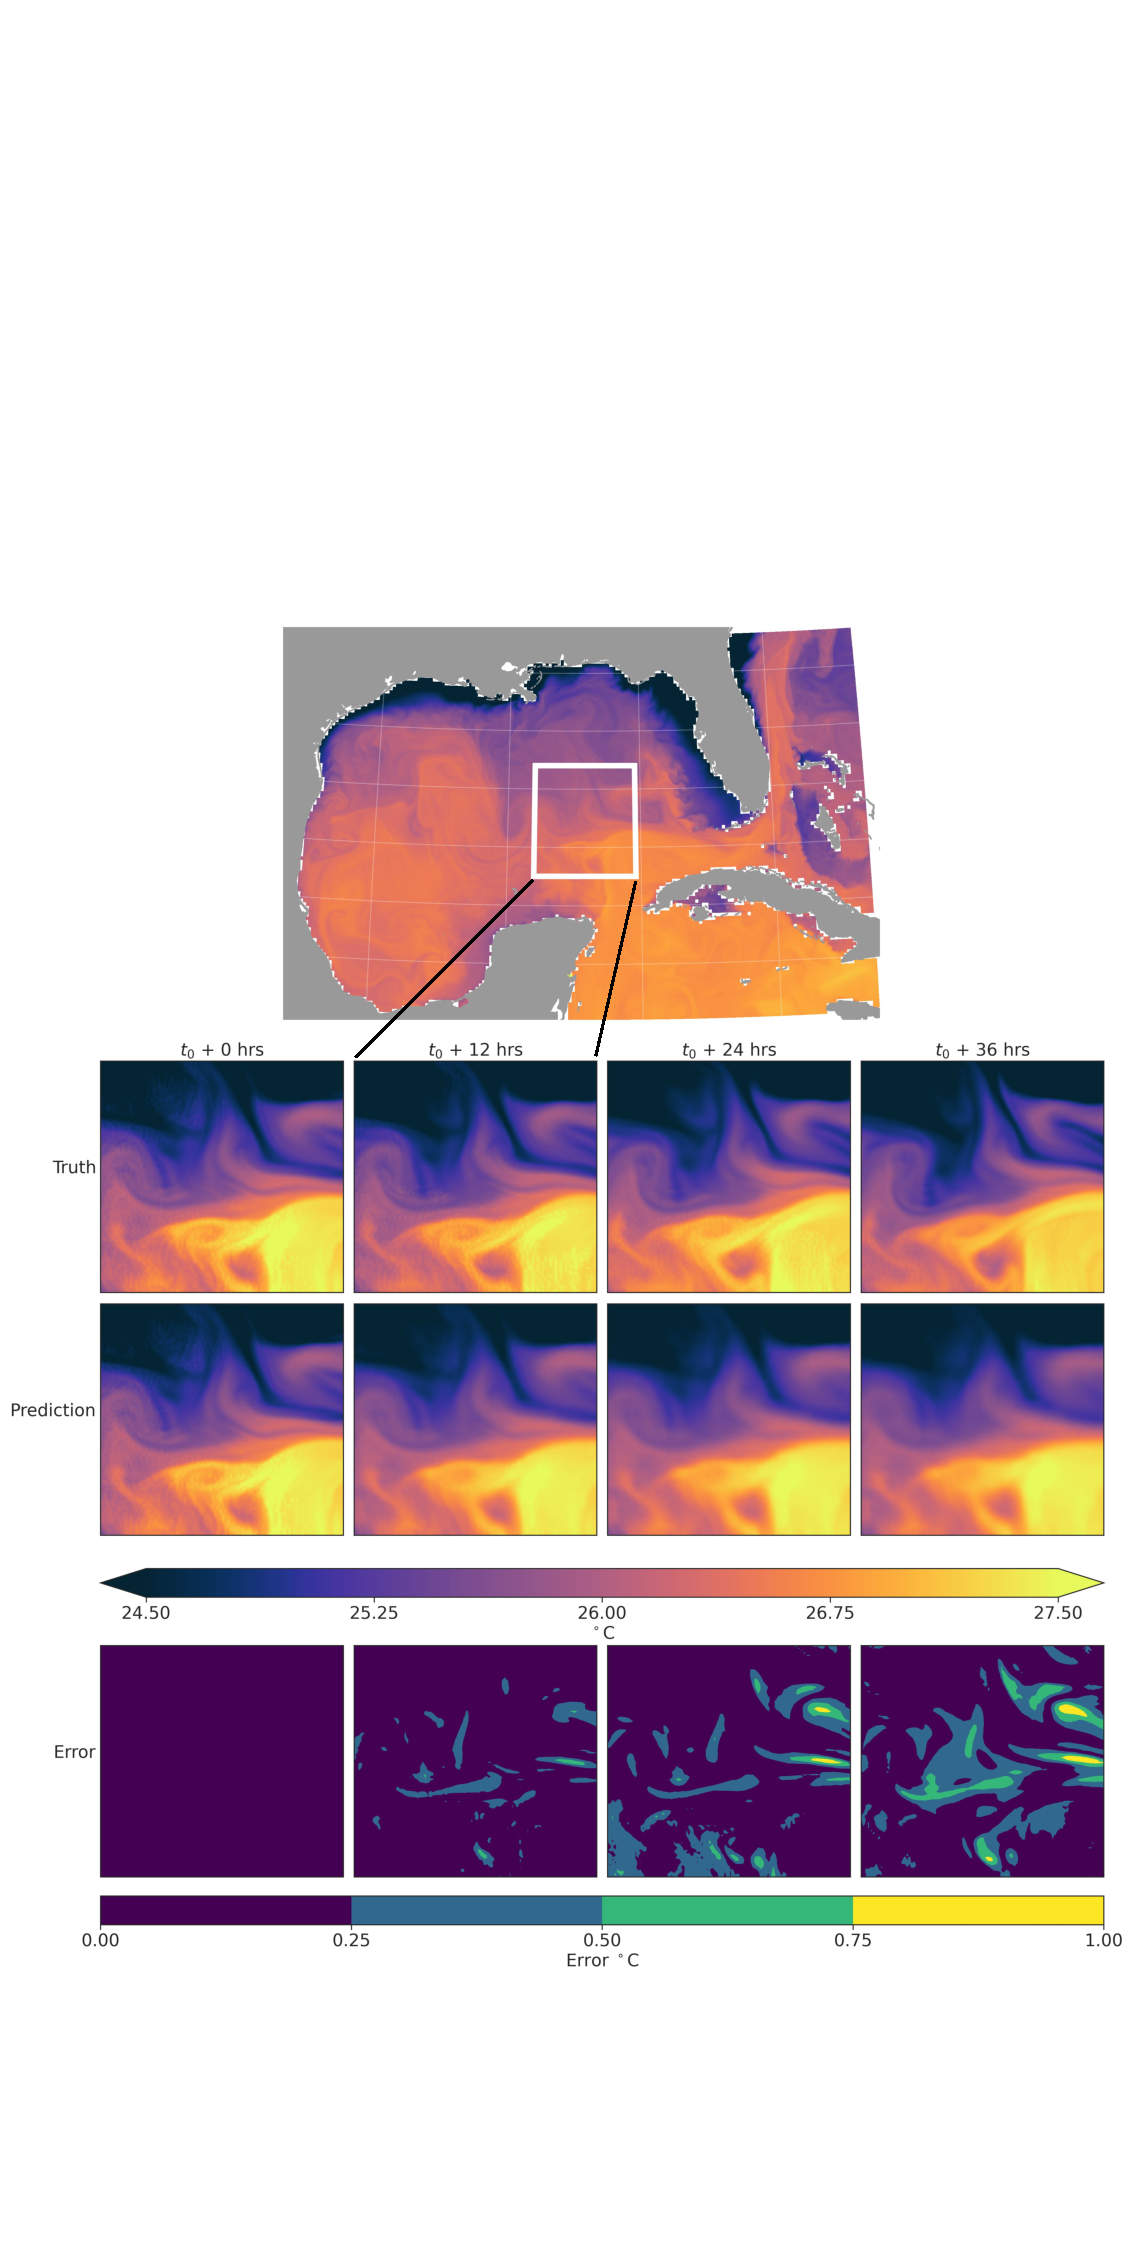
\includegraphics[width=.8\textwidth]{../figures/rc_gom_sst.pdf}
    \caption{A sample prediction of SSTs in the Gulf of Mexico at 1/25$^\circ$
        horizontal resolution.
        The upper row (Truth) shows the evolution of unseen test data from the
        Navy/HYCOM reanalysis product, and the middle row shows a prediction
        from the Reservoir Computing architecture described in
        \cref{subsec:rc}.
        The bottom row (Error) shows the absolute value of the difference between the two.
        See \cref{sec:datasets} for a description of the training and testing data
        used.
    }
    \label{fig:gom_sst}
\end{figure}


